\subsection{Mô hình XGBoost}

\subsubsection{Mô hình cho tập dữ liệu chỉ bao gồm các quan sát có cột "emailtotal" không phải giá trị null}

\begin{enumerate}[label=(\alph*)]
    \item Đầu vào mô hình là vector thu được từ phân tích thành phần chính sử dụng thuật toán PCA
    
    Ta có bảng kết quả huấn luyện mô hình:

    \begin{python}
                    precision    recall  f1-score   support

   Keeping house       0.08      0.03      0.05        58
           Other       0.00      0.00      0.00         8
         Retired       0.31      0.32      0.32       109
          School       0.08      0.07      0.07        14
Temp not working       0.00      0.00      0.00        15
Unempl, laid off       0.00      0.00      0.00        25
Working fulltime       0.59      0.78      0.67       351
Working parttime       0.22      0.09      0.12        80

        accuracy                           0.48       660
       macro avg       0.16      0.16      0.15       660
    weighted avg       0.40      0.48      0.43       660

    \end{python}

    và ma trận nhầm lẫn:

    \begin{figure}[H]
        \centering
        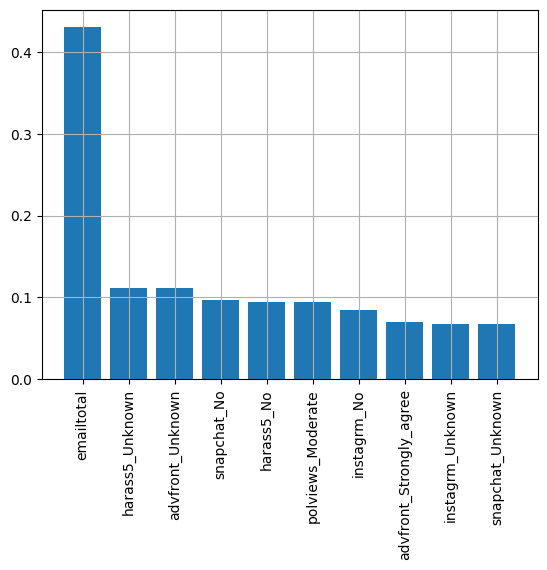
\includegraphics[width=0.6\textwidth]{figures/Thanh/Models/XGBoost/Non_null_models_Feature_Importance_XGBoost_PCA_features.png}
        \caption{Ma trận nhầm lẫn của mô hình XGBoost với vector đầu vào là vector thu được từ phân tích thành phần chính sử dụng thuật toán PCA}
        \label{fig:Non_null_models_Feature_Importance_XGBoost_PCA_features}
    \end{figure}

    Ta nhận thấy kết quả F1-score cho hai lớp làm việc toàn thời gian và đã nghỉ hưu cao hơn so với mô hình AdaBoost và có sự đồng đều về kết quả giữa các lớp hơn so với các mô hình trước.

    Ta sẽ phân tích ngược trở lại trọng số của các tham số tương ứng với các đặc trưng của vector ban đầu từ các tham số ứng với các đặc trưng của các thành phần chính:

    \begin{figure}[H]
        \centering
        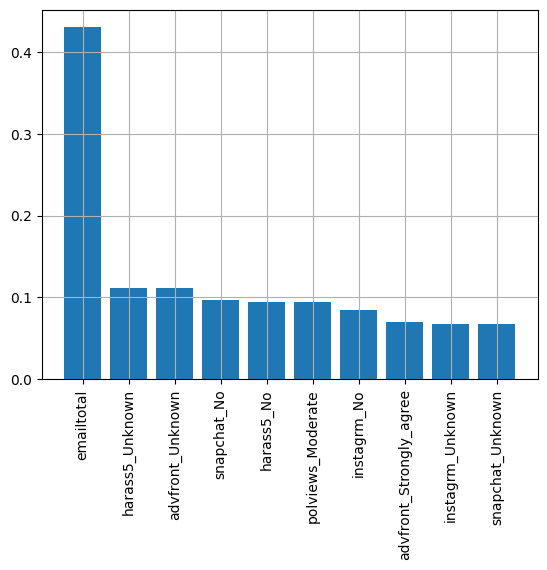
\includegraphics[width=0.6\textwidth]{figures/Thanh/Models/XGBoost/Non_null_models_Feature_Importance_XGBoost_PCA_features.png}
        \caption{Biểu đồ cột sắp xếp độ lớn giảm dần (trị tuyệt đối) tham số của các đặc trưng (mô hình với vector đầu vào là vector được phân tích thành phần chính sử dụng thuật toán PCA}
        \label{fig:Non_null_models_Feature_Importance_XGBoost_PCA_features}
    \end{figure}

    Ta có biểu đồ cột sắp xếp độ lớn giảm dần (trị tuyệt đối) tham số của các đặc trưng thể hiện ở hình \ref{fig:Non_null_models_Feature_Importance_XGBoost_PCA_features}.
    Ta nhận thấy các cột có trọng số lớn và ảnh hưởng nhiều tới các các nhãn đầu ra là emailtotal, harass5\_Unknown.

    \item Vector đầu vào là vector gốc ban đầu
    
    Ta có bảng kết quả huấn luyện mô hình:

    \begin{python}
                    precision    recall  f1-score   support

   Keeping house       0.15      0.09      0.11        58
           Other       0.00      0.00      0.00         8
         Retired       0.36      0.18      0.24       109
          School       0.20      0.14      0.17        14
Temp not working       0.00      0.00      0.00        15
Unempl, laid off       0.33      0.04      0.07        25
Working fulltime       0.57      0.85      0.68       351
Working parttime       0.21      0.09      0.12        80

        accuracy                           0.51       660
       macro avg       0.23      0.17      0.17       660
    weighted avg       0.42      0.51      0.44       660

    \end{python}

    và ma trận nhầm lẫn:

    \begin{figure}[H]
        \centering
        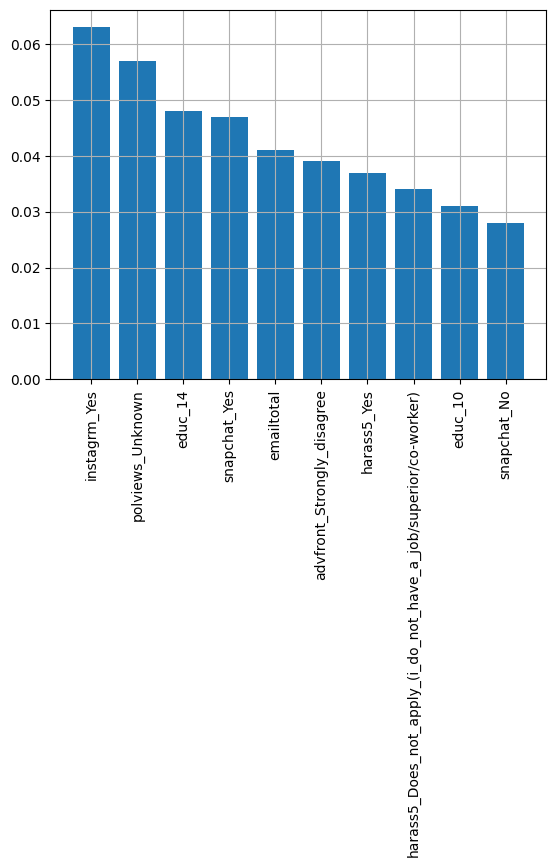
\includegraphics[width=0.6\textwidth]{figures/Thanh/Models/XGBoost/Non_null_models_Feature_Importance_XGBoost_original_features.png}
        \caption{Ma trận nhầm lẫn của mô hình XGBoost khi vector đầu vào là vector gốc ban đầu}
        \label{fig:Non_null_models_Feature_Importance_XGBoost_original_features}
    \end{figure}
    
    Ta nhận thấy kết quả phân loại không khác nhiều so với trường hợp đầu vào mô hình là vector được phân tích thành phần chính sử dụng thuật toán PCA.
    Kết quả của nhãn Keeping House, School, Unempl-laid off tăng lên và kết quả của nhãn Retired giảm đi.
    Nhưng nhìn chung khả năng phân loại của mô hình tăng lên.
    Điều này càng phản ánh sự trỗn lẫn, khó phân biệt của phân phối dữ liệu tương ứng với từng nhãn trong cột wrkstat.
    Mô hình XGBoost là một mô hình phân loại khá tốt.

    Ta sẽ phân tích ngược trở lại trọng số của các tham số tương ứng với các đặc trưng của vector ban đầu từ các tham số ứng với các đặc trưng:

    \begin{figure}[H]
        \centering
        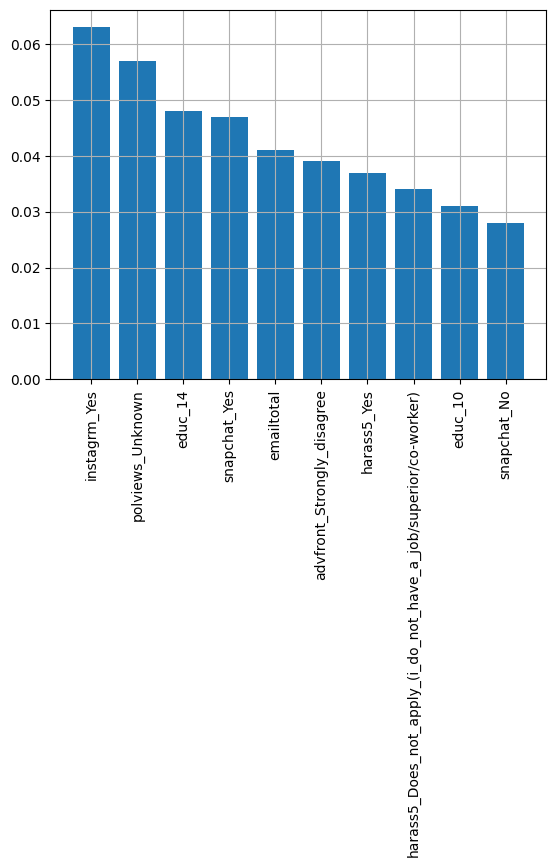
\includegraphics[width=0.6\textwidth]{figures/Thanh/Models/XGBoost/Non_null_models_Feature_Importance_XGBoost_original_features.png}
        \caption{Biểu đồ cột sắp xếp độ lớn giảm dần (trị tuyệt đối) tham số của các đặc trưng (mô hình với vector đầu vào là vector gốc ban đầu)}
        \label{fig:Non_null_models_Feature_Importance_XGBoost_original_features}
    \end{figure}
    
    Ta có biểu đồ cột sắp xếp độ lớn giảm dần (trị tuyệt đối) của các đặc trưng thể hiện ở hình \ref{fig:Non_null_models_Feature_Importance_XGBoost_original_features}.
    Ta nhận thấy các đặc trưng có trọng số lớn là instgrm\_Yes, polviews\_Unknown.
\end{enumerate}